\chapter{Didattica della programmazione}

\section{L'apprendimento}

\nt{I seguenti risultati (teoria dei magazzini di memoria) è frutto degli studi del cognitivismo.}

\begin{center}
    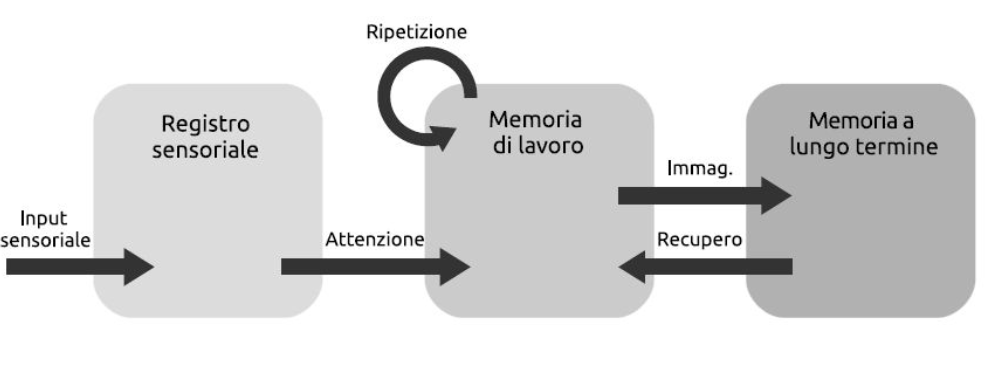
\includegraphics[scale = 0.4]{images/didattica della programmazione/Apprendimento.png}
\end{center}

\dfn{Registro sensoriale}{L'input sensoriale è ciò che viene acquisito dai 5 sensi.}

\nt{Nell'apprendimento l'input è solitamente l'udito o la vista.}

\dfn{Memoria a breve termine (o memoria di lavoro)}{Serve attenzione per passare dal registro sensoriale alla memoria di lavoro. Ha una capienza limitata in termini di spazio e tempo (circa 10 secondi, aumentabli con la ripetizione.}

\nt{Quando si sta imparando la memoria di lavoro è totalmente concentrata su un compito.}

\dfn{Memoria a lungo termine}{Ha capacità potenzialmente illimitate\footnote{Non esattamente}. Non si è coscenti di queste memorie che devono essere portate, ogni volta, nella memoria di lavoro.}

\dfn{Apprendimento}{L'apprendimento richiede che la conoscenza avviene solo quando il concetto passa dalla memoria a breve termine alla memoria a lungo termine.}

\nt{Se si "impara" una cosa, ma il giorno dopo non si riesce più a replicarla non si ha apprendimento.}

\section{La programmazione}

\dfn{Programmare}{La \newfancyglitter{programmazione} è una rappresentazione di base fatta di schemi\footnote{Problemi}, le soluzioni e le informazioni associate.}

\nt{Ciò che distingue un esperto da un principiante è la capacità di attingere a molti più schemi memorizzati nella memoria a lungo termine.}

\qs{}{Com'è possibile che l'uomo riesca a svolgere attività mentali complesse con una memoria di lavoro tanto limitata?}

\begin{itemize}
    \item Si apprende meglio quando la memoria di lavoro non è troppo vuota o troppo piena;
    \item Il carico cognitivo è legato alla memoria di lavoro;
    \item Il carico cognitivo può essere:
    \begin{enumerate}
        \item Intrinseco: imposto dal compito;
        \item Pertinente: usate per creare o modificare schemi, ma non indispensabile;
        \item Estraneo: inutile.
    \end{enumerate}
\end{itemize}

\nt{
\begin{itemize}
    \item Si deve mantenere un carico pertinente elevato;
    \item Se il carico intrinseco è elevato non si apprende\footnote{Ci si concentra sul problema, ma non sugli schemi};
    \item Se il carico cognitivo è basso ci si annoia;
    \item Se possibile conviene ridurre il carico cognitivo di compiti difficili.
\end{itemize}
}

\pagebreak

\section{Pattern}

\ex{Un abuso di pattern}{
\begin{center}
    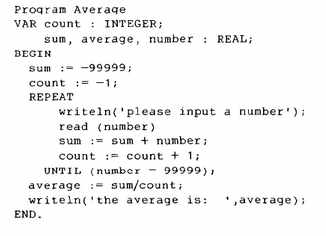
\includegraphics[scale = 0.7]{images/didattica della programmazione/Media.png}
\end{center}

Questo programma è stato scritto da uno studente che aveva intenzione di usare il pattern [Repeat Until] per risolvere il problema della media di una serie di input in cui il valore 99999 funge da guardia. Durante la progettazione lo studente si è trovato con il valore 99999 nella media (che ovviamente non deve essere incluso), motivo per cui ha dovuto inizializzare sum a -99999 (in questo modo i suoi valori si annullano)\footnote{Personalmente la ritengo una soluzione creativa, ma i docenti non sono dello stesso avviso}. Bisogna far capire allo studente che ci sono costrutti più indicati per risolvere questo problema, per esempio il while. Oltre a questo un errore è il count a - 1 che causa una divisione per 0 se si inserisce 99999 all'inizio, ma questo rappresenta un  problema successivo allo studio dei pattern\footnote{Casistica}. 
}

\ex{I pattern}{

\paragraph{Problema:} Si scriva un programma che trovi il minimo in un vettore non ordinato di dimensione nota, maggiore di 0, in cui ogni valore può raggiungere al massimo 99999.

\begin{enumerate}
    \item Input: vettore V[i], dimensione i;
    \item Si inizializza min a 99999, che andrà a trovare il minimo 
    \item Si effettua una [scansione elementare semplice] con l'indice i che viene decrementato a ogni iterazione;
    \item Durante la scansione si effettua una [Guarded-Action];
    \item Se la guardia è soddisfatta si aggiorna la variabile min;
    \item Se la guardia non è soddisfatta si continua finchè il ciclo non termina;
    \item Si stampa il valore min.
\end{enumerate}

}








